% =============================================================================
% Module 12: Weak Gravitational Lensing and Cosmic Shear
% =============================================================================
% Sources: Schneider, Kochanek & Wambsganss (2006), Part 3 (P. Schneider),
%          Sect. 2 (Principles), Sect. 5 (Mass reconstruction), Sect. 6
%          (Cosmic shear), Sect. 8 (Galaxy-galaxy lensing);
%          Bartelmann & Schneider (2001); Kaiser & Squires (1993).
% Mathematica: ../Mathematica/12_Weak_Lensing/
% =============================================================================

\chapter{Weak Gravitational Lensing and Cosmic Shear}
\label{ch:weak_lensing}

\begin{quote}
\textit{One cannot `see' the effect, nor can it be graphically displayed
easily.  Only by investigating many faint galaxy images can a signal be
extracted from the data, and the human eye is not sufficient to perform
this analysis.}
\hfill --- P.~Schneider, \textit{Weak Gravitational Lensing} (2006)
\end{quote}

\noindent
Modules~\ref{ch:lens_equation}--\ref{ch:cluster_lensing} were concerned
almost entirely with \textbf{strong} lensing: multiple images, giant
arcs, Einstein rings --- phenomena in which the Jacobian
$\Amat = \partial\vecbeta/\partial\vectheta$ differs so much from the
identity that a single source produces spectacularly distorted images.
This module treats the opposite, and far more common, regime.  In
\textbf{weak} gravitational lensing the Jacobian is very close to the
unit matrix,
\begin{equation*}
    \Amat = \begin{pmatrix} 1 - \kappab - \gammaL_1 & -\gammaL_2 \\
    -\gammaL_2 & 1 - \kappab + \gammaL_1 \end{pmatrix}
    \approx \mathbb{1}\,,
    \qquad \kappab \ll 1\,, \quad |\gammaL| \ll 1\,,
\end{equation*}
so the distortion and magnification of any \textit{individual} background
galaxy are tiny and cannot be recognized.  The lensing signal is
recovered only \textit{statistically}, by averaging the shapes of many
faint galaxies \citep{schneider_kochanek_wambsganss_2006}.

This is the natural complement to the convergence--shear formalism of
Module~\ref{ch:magnification}.  There we \textit{defined} $\kappab$,
$\gammaL$, and the Jacobian; here we learn how to \textit{measure} them
from data, and what they tell us:
\begin{itemize}[nosep]
    \item how the shape of a faint galaxy provides a noisy but unbiased
          estimate of the (reduced) shear
          ($\S$\ref{sec:wl_shapes});
    \item how the tangential shear around a mass concentration measures
          its projected mass profile
          ($\S$\ref{sec:wl_tangential}), extending the axisymmetric
          result $|\gammaL| = \bar{\kappa} - \kappab$ of
          Module~\ref{ch:axisymmetric_models};
    \item how the shear field can be inverted into a parameter-free map
          of the projected mass --- the Kaiser--Squires inversion
          ($\S$\ref{sec:wl_ks}) --- and why the \textit{mass-sheet
          degeneracy} of Module~\ref{ch:galaxy_lensing} reappears here
          ($\S$\ref{sec:wl_reduced_shear});
    \item how the coherent distortion imprinted by the large-scale
          structure --- \textit{cosmic shear} --- probes cosmology
          ($\S$\ref{sec:wl_cosmic}); and
    \item how stacking foreground--background galaxy pairs measures the
          mean mass profile of galaxies
          ($\S$\ref{sec:wl_ggl}).
\end{itemize}
This chapter expands the brief weak-lensing sketch of
$\S$\ref{sec:weak_lensing} in Module~\ref{ch:cluster_lensing} into a
self-contained treatment of the core concepts.

\medskip
\noindent
\textbf{Companion Mathematica files:}
\begin{itemize}[nosep]
    \item \mathlink{12_Weak_Lensing/weak_lensing.wl}{weak\_lensing.wl}
          --- symbolic verification of the Kaiser--Squires kernel and
          inversion, the tangential-shear relation for the SIS and point
          mass, reduced-shear invariance under the mass-sheet transform,
          and the image--ellipticity relations; tangential-shear profile
          and Kaiser--Squires schematic figures exported to
          \texttt{Figures/12\_Weak\_Lensing/}
\end{itemize}


% =====================================================================
\section{Introduction: The Weak Regime}
\label{sec:wl_intro}

In strong lensing a single source tells the whole story: from the
positions and fluxes of a handful of multiple images one constrains the
deflector.  In the weak regime, $\kappab \ll 1$ and $|\gammaL| \ll 1$,
no individual source carries a recognizable signal.  Instead, one exploits
the fact that lensing preserves surface brightness while distorting shapes:
the observed ellipticity of each faint galaxy is a sum of its (unknown)
intrinsic ellipticity and a small, coherent shear.  Because intrinsic
ellipticities are randomly oriented, they average to zero, and the mean
observed ellipticity of a local ensemble of galaxies estimates the shear
\citep{schneider_kochanek_wambsganss_2006}.

The accuracy of any weak-lensing measurement is therefore set by the
number of usable background galaxies: the statistical error on the shear
scales as $\sigma_\epsilon/\sqrt{N}$, where $\sigma_\epsilon \approx 0.3$
is the intrinsic ellipticity dispersion (``shape noise'') and $N$ is the
number of galaxies averaged over.  This is why deep imaging --- reaching
$n \sim 10$--$40$ galaxies per arcmin$^2$ --- is the fundamental
observational requirement, and why correcting the atmospheric and
telescope point-spread function (which circularizes small images) is the
central technical challenge of the field
(\citealp{schneider_kochanek_wambsganss_2006}, Part~3, Sect.~3;
\citealp{bartelmann_schneider_2001}).

Throughout this module we work in the thin-lens picture of
Module~\ref{ch:lens_equation} for individual galaxies and clusters, and
generalize to a three-dimensional deflecting mass distribution --- the
large-scale structure --- only in $\S$\ref{sec:wl_cosmic}, where the
lensing effect is described by an \textit{effective} surface mass density.


% =====================================================================
\section{Galaxy Shapes and the Shear Estimator}
\label{sec:wl_shapes}

\subsection{Complex Ellipticity}

To turn shapes into shear we first need a quantitative measure of the
shape of an image with arbitrary isophotes.  Let $I(\vectheta)$ be the
surface-brightness distribution of an isolated image.  Its centroid is
$\bar{\vectheta} = \int d^2\theta\, I\, q_I[I]\, \vectheta /
\int d^2\theta\, I\, q_I[I]$ for a suitable weight $q_I$, and the tensor
of second brightness moments is
(\citealp{schneider_kochanek_wambsganss_2006}, Part~3, eq.~6)
\begin{equation}
    Q_{ij} = \frac{\int d^2\theta\, I(\vectheta)\, q_I[I]\,
    (\theta_i - \bar\theta_i)(\theta_j - \bar\theta_j)}
    {\int d^2\theta\, I(\vectheta)\, q_I[I]}\,,
    \qquad i,j \in \{1,2\}\,.
    \label{eq:wl_Qij}
\end{equation}
The trace $Q_{11} + Q_{22}$ measures the size of the image, while the
traceless part carries the ellipticity.  One defines two complex
ellipticities
(\citealp{schneider_kochanek_wambsganss_2006}, Part~3, eq.~7)
\begin{equation}
    \boxed{
    \chi \equiv \frac{Q_{11} - Q_{22} + 2\mathrm{i}\, Q_{12}}
    {Q_{11} + Q_{22}}\,,
    \qquad
    \epsilon \equiv \frac{Q_{11} - Q_{22} + 2\mathrm{i}\, Q_{12}}
    {Q_{11} + Q_{22} + 2\left(Q_{11}Q_{22} - Q_{12}^2\right)^{1/2}}\,.
    }
    \label{eq:wl_ellipticities}
\end{equation}
Both share the same phase (that of the traceless part), so both encode the
same orientation, but they differ in modulus.  For an image with elliptical
isophotes of axis ratio $r = b/a \le 1$
(\citealp{schneider_kochanek_wambsganss_2006}, Part~3, eq.~8),
\begin{equation}
    |\chi| = \frac{1 - r^2}{1 + r^2}\,,
    \qquad
    |\epsilon| = \frac{1 - r}{1 + r}\,,
    \label{eq:wl_chi_eps_r}
\end{equation}
and the two are related by
\begin{equation}
    \epsilon = \frac{\chi}{1 + \sqrt{1 - |\chi|^2}}\,,
    \qquad
    \chi = \frac{2\epsilon}{1 + |\epsilon|^2}\,.
    \label{eq:wl_chi_eps_transform}
\end{equation}
The phase of $\chi$ and $\epsilon$ is $2\varphi$, twice the position angle
$\varphi$ of the major axis; the factor of two reflects the fact that an
ellipse maps to itself under a rotation by $180^\circ$.  It is this
``spin-2'' character that $\chi$ and $\epsilon$ share with the shear
(Module~\ref{ch:magnification}, eq.~\ref{eq:shear_spin2}).

\subsection{From Source to Image, and the Estimator}

Under the linearized lens mapping the source and image second-moment
tensors are related by $Q^{(s)} = \Amat\, Q\, \Amat^{\mathsf T}$, which in
terms of the complex ellipticity $\epsilon$ and the \textbf{reduced shear}
$g = \gammaL/(1 - \kappab)$ becomes
(\citealp{schneider_kochanek_wambsganss_2006}, Part~3, eq.~12)
\begin{equation}
    \epsilon^{(s)} = \frac{\epsilon - g}{1 - g^*\epsilon}
    \qquad (|g| \le 1)\,,
    \label{eq:wl_eps_source}
\end{equation}
with the inverse obtained by $\epsilon \leftrightarrow \epsilon^{(s)}$ and
$g \to -g$.  Now comes the key statistical assumption: faint galaxies have
no preferred orientation, so the intrinsic ellipticity averages to zero,
\begin{equation}
    \mathrm{E}\!\left[\epsilon^{(s)}\right] = 0\,.
    \label{eq:wl_random_orientation}
\end{equation}
Averaging the transformation~\eqref{eq:wl_eps_source} over intrinsic
orientations then gives the remarkable result
(\citealp{schneider_kochanek_wambsganss_2006}, Part~3, eq.~14)
\begin{equation}
    \boxed{
    \mathrm{E}[\epsilon] = g
    \qquad (|g| \le 1)\,.
    }
    \label{eq:wl_expectation_eps}
\end{equation}
\textit{Each galaxy ellipticity is an unbiased --- though very noisy ---
estimate of the local reduced shear.}  The noise is set by the intrinsic
dispersion $\sigma_\epsilon = \sqrt{\langle \epsilon^{(s)}\epsilon^{(s)*}
\rangle}$: averaging over $N$ galaxies subject to the same $g$, the
$1\sigma$ error on the mean is
$\approx \sigma_\epsilon/\sqrt{N}$
(\citealp{schneider_kochanek_wambsganss_2006}, Part~3, eq.~15).

In the proper weak regime, $\kappab \ll 1$ and $|\gammaL| \ll 1$, the
reduced shear and shear coincide, and one has the useful chain
(\citealp{schneider_kochanek_wambsganss_2006}, Part~3, eq.~16)
\begin{equation}
    \gammaL \approx g \approx \langle \epsilon \rangle
    \approx \frac{\langle \chi \rangle}{2}\,.
    \label{eq:wl_weak_chain}
\end{equation}
The factor $\tfrac{1}{2}$ between $\langle\chi\rangle$ and the shear
follows directly from~\eqref{eq:wl_chi_eps_r}: for small distortions
$|\chi| \approx 2|\epsilon|$.

\begin{remark}
Shape noise is irreducible: even with perfect measurements, the finite
intrinsic ellipticity dispersion $\sigma_\epsilon$ sets a floor on the
achievable accuracy.  The only levers are the number density $n$ of usable
galaxies and the survey area.  Increasing $n$ means going deeper, which
also pushes to higher-redshift (more strongly lensed) sources --- a double
benefit that motivates deep, wide imaging surveys.
\end{remark}


% =====================================================================
\section{Tangential and Cross Shear}
\label{sec:wl_tangential}

\subsection{Definitions}

The shear is not a vector: under a rotation of the coordinate frame by
$\phi$ its complex representation is multiplied by $e^{-2\mathrm{i}\phi}$,
not $e^{-\mathrm{i}\phi}$.  It is a \textbf{spin-2} (polar) quantity, like
linear polarization.  Relative to a chosen direction $\phi$ one defines
the \textbf{tangential} and \textbf{cross} components
(\citealp{schneider_kochanek_wambsganss_2006}, Part~3, eq.~17)
\begin{equation}
    \boxed{
    \gammaL_{\mathrm t} = -\mathrm{Re}\!\left(\gammaL\, e^{-2\mathrm{i}\phi}\right)\,,
    \qquad
    \gammaL_\times = -\mathrm{Im}\!\left(\gammaL\, e^{-2\mathrm{i}\phi}\right)\,,
    }
    \label{eq:wl_tangential_cross}
\end{equation}
and identically for the ellipticity components $\epsilon_{\mathrm t},
\epsilon_\times$.  Taking $\phi$ to be the polar angle of the point
relative to a chosen center, $\gammaL_{\mathrm t} > 0$ describes a shear
oriented \textit{tangentially} (an image stretched perpendicular to the
line to the center), and $\gammaL_{\mathrm t} < 0$ a radial stretch.  The
sign in~\eqref{eq:wl_tangential_cross} is fixed precisely so that a
circular mass concentration --- which stretches background images
tangentially --- produces a \textit{positive} $\gammaL_{\mathrm t}$.
For a circularly symmetric deflector the shear is purely tangential at
every point, so $\gammaL_\times = 0$; a non-zero cross component averaged
over many pairs is a classic null test for systematics (its expectation
vanishes by parity, $\S$\ref{sec:wl_cosmic}).

\subsection{Mean Tangential Shear and the Projected Mass}

For a \textbf{circularly symmetric} lens we already know from
Module~\ref{ch:axisymmetric_models}
(eq.~\ref{eq:gamma_circular}) that
$\gammaL_{\mathrm t}(\theta) = \bar\kappa(\theta) - \kappab(\theta)$,
the mean convergence interior to $\theta$ minus the local convergence.
A beautiful result of Schneider (2006) is that a nearly identical relation
holds for the \textit{azimuthal average} of a completely general,
non-symmetric mass distribution.  Starting from Gauss's theorem applied to
the deflection potential $\psiL$ (with $\nabla^2\psiL = 2\kappab$) and
differentiating the enclosed dimensionless mass
$m(\theta) = \pi^{-1}\!\int_{|\vartheta| \le \theta} d^2\vartheta\,
\kappab(\vartheta) = \theta^2\bar\kappa(\theta)$ with respect to $\theta$,
one obtains
(\citealp{schneider_kochanek_wambsganss_2006}, Part~3, eq.~24)
\begin{equation}
    \boxed{
    \langle \gammaL_{\mathrm t}\rangle(\theta)
    = \bar\kappa(\theta) - \langle\kappab\rangle(\theta)\,,
    }
    \label{eq:wl_mean_tangential}
\end{equation}
where $\langle\cdot\rangle(\theta)$ denotes the average over the circle of
radius $\theta$ and $\bar\kappa(\theta)$ the mean convergence inside it
(Bartelmann 1995).  The immediate and powerful implication:
\textit{from the tangential shear averaged on concentric circles one
recovers the azimuthally-averaged mass profile of any lens, symmetric or
not.}

It is customary to write this in physical units.  Multiplying
by the critical surface mass density $\Sigmacr$
(Module~\ref{ch:lens_equation}) and using $\kappab = \Sigma/\Sigmacr$,
\begin{equation}
    \gammaL_{\mathrm t}(\theta)\,\Sigmacr
    = \bar\Sigma(<\theta) - \Sigma(\theta)
    \equiv \Delta\Sigma(\theta)\,,
    \label{eq:wl_DeltaSigma}
\end{equation}
the \textbf{excess surface mass density} $\Delta\Sigma$: the mean surface
density inside radius $\theta$ minus that at $\theta$.  Equation
\eqref{eq:wl_DeltaSigma} is the workhorse of cluster and galaxy--galaxy
weak lensing --- the observable tangential shear translates directly into
a projected mass profile.

\begin{example}
\textbf{Tangential shear of an SIS.}
For the singular isothermal sphere (Module~\ref{ch:axisymmetric_models},
eqs.~\ref{eq:sis_kappa}--\ref{eq:sis_mean_kappa}) we have
$\kappab = \thetaE/(2\theta)$ and $\bar\kappa = \thetaE/\theta$, so
\begin{equation}
    \gammaL_{\mathrm t}(\theta) = \bar\kappa - \kappab
    = \frac{\thetaE}{\theta} - \frac{\thetaE}{2\theta}
    = \frac{\thetaE}{2\theta}\,.
    \label{eq:wl_sis_gammat}
\end{equation}
The tangential shear falls off as $\theta^{-1}$, exactly tracing the
$\Sigma \propto \theta^{-1}$ isothermal profile.  For a point mass,
$\kappab = 0$ (away from the origin) and
$\gammaL_{\mathrm t} = \bar\kappa = \thetaE^2/\theta^2$.  Both are verified
in \mathlink{12_Weak_Lensing/weak_lensing.wl}{weak\_lensing.wl}.
\end{example}


% =====================================================================
\section{Reduced Shear and the Mass-Sheet Degeneracy}
\label{sec:wl_reduced_shear}

Galaxy ellipticities measure not the shear $\gammaL$ but the
\textbf{reduced shear} $g = \gammaL/(1 - \kappab)$
(eq.~\ref{eq:wl_expectation_eps}).  This has a profound consequence.
Consider the transformation, for an arbitrary constant $\lambda$,
(\citealp{schneider_kochanek_wambsganss_2006}, Part~3, eq.~51)
\begin{equation}
    \kappab(\vectheta) \;\longrightarrow\;
    \kappab'(\vectheta) = \lambda\,\kappab(\vectheta) + (1 - \lambda)\,,
    \qquad
    1 - \kappab' = \lambda\,(1 - \kappab)\,.
    \label{eq:wl_mst}
\end{equation}
Since the shear is the traceless part of the same Hessian that gives the
convergence, adding a \textit{uniform sheet} of convergence $(1-\lambda)$
leaves the shear rescaled, $\gammaL \to \gammaL' = \lambda\gammaL$, and
therefore
\begin{equation}
    \boxed{
    g' = \frac{\gammaL'}{1 - \kappab'}
    = \frac{\lambda\gammaL}{\lambda(1 - \kappab)}
    = \frac{\gammaL}{1 - \kappab} = g\,.
    }
    \label{eq:wl_g_invariant}
\end{equation}
The reduced shear --- and hence every ellipticity measurement --- is
\textit{invariant} under~\eqref{eq:wl_mst}.  This is the weak-lensing face
of the \textbf{mass-sheet degeneracy} introduced in
Module~\ref{ch:galaxy_lensing}: from shear data alone the convergence is
determined only up to the one-parameter family~\eqref{eq:wl_mst}.  In the
Kaiser--Squires inversion below it appears as an undetermined additive
constant $\kappab_0$.

The degeneracy also rescales the magnification.  With
$\mu^{-1} = (1 - \kappab)^2 - |\gammaL|^2$
(Module~\ref{ch:magnification},
eq.~\ref{eq:magnification_formula}), the transform~\eqref{eq:wl_mst} gives
\begin{equation}
    \mu \;\longrightarrow\; \mu' = \lambda^{-2}\,\mu\,,
    \label{eq:wl_mu_rescale}
\end{equation}
which is why \textit{magnification} information --- from the lensing-induced
change in background number counts,
$n(>S)/n_0(>S) \approx 1 + 2(\alpha - 1)\kappab$ in the weak limit
(\citealp{schneider_kochanek_wambsganss_2006}, Part~3, eq.~27) --- can in
principle break the degeneracy that shear alone cannot.  Both invariances
are checked symbolically in
\mathlink{12_Weak_Lensing/weak_lensing.wl}{weak\_lensing.wl}.


% =====================================================================
\section{Cluster Mass Reconstruction}
\label{sec:wl_ks}

We now come to the discovery that launched quantitative weak lensing:
from a measured shear field one can reconstruct a \textbf{parameter-free
map of the projected mass}, with no assumption of symmetry
\citep{kaiser_squires_1993}.

\subsection{The Kaiser--Squires Inversion}

The convergence and shear are both linear (second-derivative) functionals
of the single potential $\psiL$
(Module~\ref{ch:magnification}), so they are related to each other by a
non-local convolution.  Explicitly
(\citealp{schneider_kochanek_wambsganss_2006}, Part~3, eq.~41)
\begin{equation}
    \gammaL(\vectheta) = \frac{1}{\pi}\int_{\mathbb{R}^2}
    d^2\theta'\; \mathcal{D}(\vectheta - \vectheta')\,
    \kappab(\vectheta')\,,
    \qquad
    \mathcal{D}(\vectheta) \equiv
    -\frac{\theta_1^2 - \theta_2^2 + 2\mathrm{i}\,\theta_1\theta_2}
    {|\vectheta|^4}
    = \frac{-1}{(\theta_1 - \mathrm{i}\,\theta_2)^2}\,.
    \label{eq:wl_ks_forward}
\end{equation}
The complex kernel $\mathcal{D}$ is nothing but the shear produced by a
point mass.  In Fourier space the convolution becomes a product,
$\hat\gammaL(\boldsymbol\ell) = \pi^{-1}\hat{\mathcal D}(\boldsymbol\ell)\,
\hat\kappab(\boldsymbol\ell)$, with
(\citealp{schneider_kochanek_wambsganss_2006}, Part~3, eq.~43)
\begin{equation}
    \hat{\mathcal D}(\boldsymbol\ell)
    = \pi\,\frac{\ell_1^2 - \ell_2^2 + 2\mathrm{i}\,\ell_1\ell_2}
    {|\boldsymbol\ell|^2}
    = \pi\, e^{2\mathrm{i}\beta_\ell}\,,
    \qquad
    \hat{\mathcal D}\,\hat{\mathcal D}^* = \pi^2\,,
    \label{eq:wl_Dhat}
\end{equation}
where $\beta_\ell$ is the polar angle of $\boldsymbol\ell$.  Because
$|\hat{\mathcal D}|^2 = \pi^2$ is a constant, the relation inverts
trivially, $\hat\kappab = \pi^{-1}\hat\gammaL\,\hat{\mathcal D}^*$
(for $\boldsymbol\ell \neq 0$), and transforming back to real space yields
the \textbf{Kaiser--Squires inversion}
(\citealp{schneider_kochanek_wambsganss_2006}, Part~3, eq.~44;
\citealp{kaiser_squires_1993})
\begin{equation}
    \boxed{
    \kappab(\vectheta) - \kappab_0
    = \frac{1}{\pi}\int_{\mathbb{R}^2} d^2\theta'\;
    \mathrm{Re}\!\left[\mathcal{D}^*(\vectheta - \vectheta')\,
    \gammaL(\vectheta')\right].
    }
    \label{eq:wl_ks_inversion}
\end{equation}
Since the observed shear can be estimated at galaxy positions
(via eq.~\ref{eq:wl_expectation_eps}), \eqref{eq:wl_ks_inversion} converts
a measured shear map into a mass map.

\begin{remark}
Three features of~\eqref{eq:wl_ks_inversion} deserve emphasis, all
verified in \mathlink{12_Weak_Lensing/weak_lensing.wl}{weak\_lensing.wl}:
\begin{enumerate}[nosep]
    \item \textbf{The additive constant $\kappab_0$.}
          $\hat{\mathcal D}$ is undefined at $\boldsymbol\ell = 0$, so the
          mean (DC) mode of $\kappab$ is unconstrained.  This is exactly
          the mass-sheet degeneracy~\eqref{eq:wl_mst}: a uniform sheet
          produces no shear.
    \item \textbf{Reduced shear, not shear.}
          What is measured is $g$, not $\gammaL$; in ``weak'' weak lensing
          $\gammaL \approx g$, but in the non-linear inner regions of
          clusters one must solve the integral equation
          \begin{equation*}
              \kappab - \kappab_0 = \frac{1}{\pi}\int d^2\theta'\,
              \left[1 - \kappab(\vectheta')\right]
              \mathrm{Re}\!\left[\mathcal{D}^*(\vectheta - \vectheta')\,
              g(\vectheta')\right]
          \end{equation*}
          iteratively
          (\citealp{schneider_kochanek_wambsganss_2006}, Part~3, eq.~50).
    \item \textbf{Smoothing.}
          A naive discrete sum over galaxies has formally infinite
          variance (the $\theta^{-2}$ kernel); a smoothing kernel is
          required to obtain a finite-variance mass estimator.
\end{enumerate}
\end{remark}

\subsection{Aperture Mass}
\label{sec:wl_apmass}

The undetermined constant $\kappab_0$ motivates a statistic that is
\textit{immune} to the mass-sheet degeneracy: the \textbf{aperture mass}
(\citealp{schneider_kochanek_wambsganss_2006}, Part~3, eq.~108)
\begin{equation}
    M_{\mathrm{ap}}(\theta) = \int d^2\vartheta\;
    Q(|\vartheta|)\,\gammaL_{\mathrm t}(\vartheta)\,,
    \label{eq:wl_Map}
\end{equation}
a weighted integral of the tangential shear within an aperture of radius
$\theta$, with $Q$ a weight function of compact support.  If $Q$ is
derived from a \textit{compensated} filter $U$ (one with
$\int d^2\vartheta\, U = 0$), then $M_{\mathrm{ap}}$ can equivalently be
written as $\int d^2\vartheta\, U(|\vartheta|)\,\kappab(\vartheta)$: because
$U$ integrates to zero, adding a uniform sheet $\kappab_0$ contributes
nothing, so $M_{\mathrm{ap}}$ is invariant under~\eqref{eq:wl_mst}.
Since it is built from the observable $\gammaL_{\mathrm t}$ directly, it
requires no inversion, and --- as we see next --- doubles as a clean
cosmic-shear statistic and as a matched filter for detecting mass
concentrations by their shear alone.

\begin{figure}[ht]
    \centering
    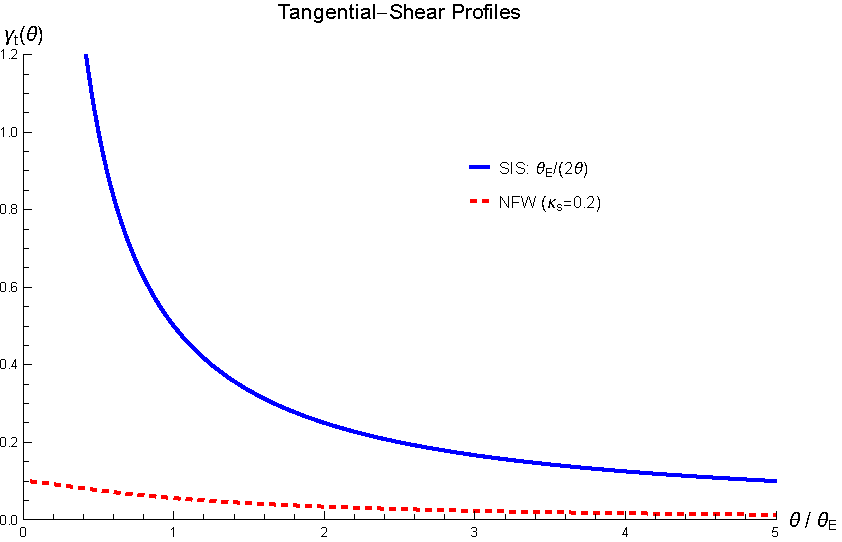
\includegraphics[width=0.82\textwidth]{../Figures/12_Weak_Lensing/tangential_shear_profiles.pdf}
    \caption{Tangential-shear profiles $\gammaL_{\mathrm t}(\theta)$ for
    two axisymmetric lenses, illustrating
    eq.~\eqref{eq:wl_mean_tangential}.  \textbf{Solid:} the singular
    isothermal sphere, $\gammaL_{\mathrm t} = \thetaE/(2\theta)$
    (eq.~\ref{eq:wl_sis_gammat}), with $\thetaE = 1$.  \textbf{Dashed:} an
    NFW halo (Module~\ref{ch:axisymmetric_models},
    eq.~\ref{eq:nfw_gamma}) with $\kappa_s = 0.2$ and scale
    $\theta_s = 1$; the NFW tangential shear turns over near the scale
    radius, unlike the featureless power law of the SIS.  The measurable
    $\gammaL_{\mathrm t}$ maps directly to the excess surface mass density
    $\Delta\Sigma$ (eq.~\ref{eq:wl_DeltaSigma}).  Generated by
    \texttt{weak\_lensing.wl}.}
    \label{fig:wl_tangential}
\end{figure}


% =====================================================================
\section{Cosmic Shear: Lensing by the Large-Scale Structure}
\label{sec:wl_cosmic}

So far the deflector has been a single, localized mass (galaxy or cluster)
in a thin lens plane.  But light bundles from distant galaxies are
distorted continuously by \textit{all} the inhomogeneous matter along the
line of sight --- the large-scale structure (LSS).  This produces a weak,
spatially coherent distortion of galaxy shapes across the sky called
\textbf{cosmic shear}, whose statistics directly probe the matter
distribution and hence cosmology (Gunn 1967; Blandford et al.\ 1991;
\citealp{schneider_kochanek_wambsganss_2006}, Part~3, Sect.~6).

\subsection{The Effective Convergence}

For a three-dimensional deflecting mass distribution, working to first
order in the Newtonian potential $\Phi$ (the Born approximation, i.e.\
integrating along the unperturbed ray), the distortion is still described
by a Jacobian $\Amat_{ij} = \delta_{ij} - \psiL_{,ij}$ with an
\textit{effective} deflection potential.  Its convergence is a
line-of-sight integral of the fractional density contrast
$\delta = \Delta\rho/\bar\rho$, weighted by the geometric lensing
efficiency
(\citealp{schneider_kochanek_wambsganss_2006}, Part~3, eq.~93)
\begin{equation}
    \kappab(\vectheta)
    = \frac{3 H_0^2\,\Omegam}{2\speedoflight^2}
    \int_0^{w_h} dw\; g(w)\, f_K(w)\,
    \frac{\delta\!\left(f_K(w)\vectheta,\, w\right)}{a(w)}\,,
    \label{eq:wl_kappa_eff}
\end{equation}
where $w$ is comoving distance, $a$ the scale factor, $f_K$ the comoving
angular-diameter distance, and $g(w) = \int_w^{w_h} dw'\, p_w(w')\,
f_K(w'-w)/f_K(w')$ is the source-averaged efficiency factor.  Two features
are worth noting: $\kappab \propto \Omegam$, because lensing responds to
the physical density contrast $\Delta\rho \propto \Omegam\,\delta$, not to
$\delta$ alone; and $\kappab$ can be negative, since $\delta$ can be
(unlike the surface density of a real cluster).

\subsection{The Convergence Power Spectrum}

Because $\delta$ is a realization of a random field, the observables are
statistical.  Applying Limber's equation to the
projection~\eqref{eq:wl_kappa_eff} relates the \textbf{convergence power
spectrum} $P_\kappa(\ell)$ to the three-dimensional matter power spectrum
$P_\delta(k)$
(\citealp{schneider_kochanek_wambsganss_2006}, Part~3, eq.~99)
\begin{equation}
    \boxed{
    P_\kappa(\ell) = \frac{9 H_0^4\,\Omegam^2}{4\speedoflight^4}
    \int_0^{w_h} dw\;
    \frac{g^2(w)}{a^2(w)}\,
    P_\delta\!\left(\frac{\ell}{f_K(w)},\, w\right).
    }
    \label{eq:wl_Pkappa}
\end{equation}
The shear power spectrum equals the convergence power spectrum, since
$\hat\gammaL(\boldsymbol\ell) = e^{2\mathrm{i}\beta_\ell}\,
\hat\kappab(\boldsymbol\ell)$ from~\eqref{eq:wl_Dhat} and $|e^{2\mathrm
i\beta_\ell}| = 1$.  The strong prefactor makes the cosmic-shear amplitude
scale roughly as $\sigma_8\,\Omegam^{0.5}$ --- the same near-degenerate
combination that governs cluster abundances --- so cosmic shear is a
premier probe of the clustering amplitude of matter
\citep{schneider_kochanek_wambsganss_2006}.

\subsection{Two-Point Statistics}

$P_\kappa$ is not measured directly; what one estimates from a shear
catalogue are real-space two-point functions.  Using the tangential and
cross components~\eqref{eq:wl_tangential_cross} defined with respect to the
line connecting each galaxy pair, one forms the two \textbf{shear
correlation functions}
(\citealp{schneider_kochanek_wambsganss_2006}, Part~3, eqs.~104--105)
\begin{equation}
    \xi_\pm(\theta)
    = \langle\gammaL_{\mathrm t}\gammaL_{\mathrm t}\rangle(\theta)
    \pm \langle\gammaL_\times\gammaL_\times\rangle(\theta)
    = \int_0^\infty \frac{d\ell\,\ell}{2\pi}\,
    J_{0,4}(\ell\theta)\, P_\kappa(\ell)\,,
    \label{eq:wl_xipm}
\end{equation}
with $J_0$ for $\xi_+$ and $J_4$ for $\xi_-$.  The mixed correlator
$\xi_\times = \langle\gammaL_{\mathrm t}\gammaL_\times\rangle$ vanishes by
parity: under a reflection $\gammaL_{\mathrm t}\to\gammaL_{\mathrm t}$ but
$\gammaL_\times \to -\gammaL_\times$, so a non-zero $\xi_\times$ (or a
``B-mode'' signal) flags residual systematics.  The correlation functions
are the preferred observable because, unlike aperture statistics, they can
be evaluated over gaps and masked regions --- one simply uses every galaxy
pair at a given separation.  The aperture-mass dispersion
$\langle M_{\mathrm{ap}}^2\rangle(\theta)$ built from the
statistic~\eqref{eq:wl_Map} is a particularly clean summary, because its
filter is so narrow that it probes $P_\kappa$ at essentially a single
multipole $\ell \sim 5/\theta$
(\citealp{schneider_kochanek_wambsganss_2006}, Part~3, eq.~109).

\begin{remark}
\textbf{Tomography.}  Splitting the source galaxies into photometric-redshift
bins and measuring $\xi_\pm$ within and between bins gives the redshift
evolution of the matter power spectrum through the changing efficiency
$g(w)$ in~\eqref{eq:wl_Pkappa}.  This ``weak-lensing tomography'' turns a
projected 2-D measurement into a partially 3-D probe, and is central to
the dark-energy programs of Stage-IV surveys.
\end{remark}


% =====================================================================
\section{Galaxy--Galaxy Lensing}
\label{sec:wl_ggl}

A single galaxy is far too weak a lens to detect individually --- the
signal-to-noise of an SIS detection scales as $S/N \propto
\thetaE\sqrt{n}\,/\sigma_\epsilon$, which for a galaxy
($\sigma_v \lesssim 200$~km\,s$^{-1}$) is hopeless
(\citealp{schneider_kochanek_wambsganss_2006}, Part~3, eq.~19).  But the
signal of \textit{many} galaxies can be stacked.  In the mean, a
background galaxy behind a foreground (lens) galaxy is stretched
tangentially about it, so the mean tangential ellipticity of background
sources, binned by the foreground--background separation $\theta$,
measures the mean tangential shear $\gammaL_{\mathrm t}(\theta)$ ---
and hence, through eq.~\eqref{eq:wl_DeltaSigma}, the \textit{average}
projected mass profile of the lens galaxies
(\citealp{schneider_kochanek_wambsganss_2006}, Part~3, Sect.~8.2;
first detected by Brainerd et al.\ 1996).

Because a single galaxy's halo cannot be mapped, one parametrizes the
lens population and fits.  A standard choice is a \textbf{truncated
isothermal sphere}: an isothermal $\rho \propto r^{-2}$ core turning to
$\rho \propto r^{-4}$ beyond a truncation radius $s$, with the velocity
dispersion and truncation scaled to luminosity via the
Faber--Jackson / Tully--Fisher relations,
\begin{equation}
    \sigma = \sigma_* \left(\frac{L}{L_*}\right)^{\beta/2},
    \qquad
    s = s_* \left(\frac{L}{L_*}\right)^{\eta},
    \qquad
    M \propto \sigma^2 s\,.
    \label{eq:wl_ggl_scaling}
\end{equation}
Fitting the stacked $\gammaL_{\mathrm t}(\theta)$ constrains
$(\sigma_*, s_*, \beta, \eta)$ and thereby the mass, extent, and
luminosity scaling of galaxy dark-matter haloes out to radii far beyond
the reach of stellar or gas dynamics.  The first detection
(Brainerd et al.\ 1996) yielded $\sigma_* \approx 160$~km\,s$^{-1}$ for an
$L_*$ galaxy; modern surveys stack millions of lenses and split them by
colour, stellar mass, and environment.  On larger scales the same
measurement transitions into a probe of the galaxy--mass cross-correlation
(the ``bias'' of galaxies relative to the underlying matter).


% =====================================================================
\section{Summary}
\label{sec:wl_summary}

\begin{itemize}
    \item \textbf{Weak regime:} $\kappab \ll 1$, $|\gammaL| \ll 1$, so
          $\Amat \approx \mathbb{1}$.  No individual source shows a
          recognizable signal; the shear is recovered only statistically,
          by averaging galaxy shapes, with error
          $\sim\sigma_\epsilon/\sqrt{N}$ set by shape noise.

    \item \textbf{Shear estimator:} the complex ellipticities $\chi,
          \epsilon$ (eq.~\ref{eq:wl_ellipticities}) are spin-2 shape
          measures.  With randomly oriented intrinsic ellipticities,
          $\mathrm{E}[\epsilon] = g$, the reduced shear --- each galaxy is
          an unbiased, noisy shear estimate.  In the weak limit
          $\gammaL \approx g \approx \langle\epsilon\rangle \approx
          \langle\chi\rangle/2$.

    \item \textbf{Tangential shear:} $\gammaL_{\mathrm t} =
          -\mathrm{Re}(\gammaL e^{-2\mathrm i\phi})$; averaged on circles,
          $\langle\gammaL_{\mathrm t}\rangle = \bar\kappa -
          \langle\kappab\rangle$ for \textit{any} mass distribution
          (eq.~\ref{eq:wl_mean_tangential}), so
          $\gammaL_{\mathrm t}\Sigmacr = \Delta\Sigma$ measures the
          projected mass profile.  For the SIS,
          $\gammaL_{\mathrm t} = \thetaE/(2\theta)$.

    \item \textbf{Mass-sheet degeneracy:} $g = \gammaL/(1-\kappab)$ is
          invariant under $\kappab \to \lambda\kappab + (1-\lambda)$,
          $\gammaL \to \lambda\gammaL$ (with $\mu \to \lambda^{-2}\mu$),
          so shear determines $\kappab$ only up to an additive constant.
          Magnification (number counts) can break it.

    \item \textbf{Kaiser--Squires:} $\gammaL$ and $\kappab$ are related by
          convolution with $\mathcal{D}(\vectheta) =
          -1/(\theta_1 - \mathrm i\theta_2)^2$; because
          $|\hat{\mathcal D}|^2 = \pi^2$, this inverts to
          $\kappab - \kappab_0 = \pi^{-1}\!\int
          \mathrm{Re}[\mathcal D^*\gammaL]\,d^2\theta'$
          (eq.~\ref{eq:wl_ks_inversion}), a parameter-free mass map.  The
          aperture mass $M_{\mathrm{ap}}$ is a mass-sheet-invariant
          alternative.

    \item \textbf{Cosmic shear:} LSS distorts galaxy shapes coherently; the
          effective convergence~\eqref{eq:wl_kappa_eff} has power spectrum
          $P_\kappa \propto \Omegam^2\!\int\! (g^2/a^2)\, P_\delta$
          (eq.~\ref{eq:wl_Pkappa}), measured via $\xi_\pm(\theta) =
          \int (d\ell\,\ell/2\pi) J_{0,4}(\ell\theta) P_\kappa$.  Amplitude
          $\sim \sigma_8\,\Omegam^{0.5}$; tomography adds redshift
          information.

    \item \textbf{Galaxy--galaxy lensing:} stacking foreground--background
          pairs measures the mean $\gammaL_{\mathrm t}$ and hence the
          average galaxy mass profile (truncated isothermal,
          eq.~\ref{eq:wl_ggl_scaling}), extending to a probe of galaxy
          bias on large scales.
\end{itemize}


% =====================================================================
\section{Problems}
\label{sec:wl_problems}

\begin{exercise}
\label{ex:wl_mst}
\textbf{(Reduced shear and the mass-sheet degeneracy.)}
The mass-sheet transform is $\kappab \to \kappab' = \lambda\kappab +
(1-\lambda)$, $\gammaL \to \gammaL' = \lambda\gammaL$, for constant
$\lambda$.
\begin{enumerate}[label=(\alph*)]
    \item Show that the reduced shear $g = \gammaL/(1-\kappab)$ is
          invariant under this transform.
    \item Using $\mu^{-1} = (1-\kappab)^2 - |\gammaL|^2$, show that the
          magnification transforms as $\mu \to \lambda^{-2}\mu$.
    \item Explain why a purely local measurement of galaxy ellipticities
          cannot break the degeneracy, and name one observable that can.
    \item Why is the transform called a ``mass sheet''?  Compute the
          convergence of a uniform sheet
          $\kappab(\vectheta) = 1-\lambda$ and its shear.
\end{enumerate}
Verify with
\solnlink{12_Weak_Lensing/problems\_12.wl}{problems\_12.wl}.
\end{exercise}

\begin{exercise}
\label{ex:wl_tangential}
\textbf{(Tangential shear and the projected mass.)}
\begin{enumerate}[label=(\alph*)]
    \item For the SIS with $\kappab(\theta) = \thetaE/(2\theta)$, compute
          the mean convergence $\bar\kappa(\theta)$ and show that the
          tangential shear is $\gammaL_{\mathrm t}(\theta) =
          \bar\kappa - \kappab = \thetaE/(2\theta)$.
    \item For a point mass, $\kappab = 0$ away from the origin.  What is
          $\gammaL_{\mathrm t}(\theta)$?  Contrast the radial fall-off of
          $\gammaL_{\mathrm t}$ for the point mass and the SIS.
    \item Starting from $\langle\gammaL_{\mathrm t}\rangle = \bar\kappa -
          \langle\kappab\rangle$ (eq.~\ref{eq:wl_mean_tangential}), show
          that in physical units the observable tangential shear equals
          the excess surface mass density,
          $\gammaL_{\mathrm t}\Sigmacr = \bar\Sigma(<\theta) -
          \Sigma(\theta)$.
    \item For an NFW halo, sketch $\gammaL_{\mathrm t}(\theta)$ using
          Module~\ref{ch:axisymmetric_models} (eq.~\ref{eq:nfw_gamma}) and
          explain qualitatively why it turns over near $\theta_s$, unlike
          the SIS.
\end{enumerate}
Verify with
\solnlink{12_Weak_Lensing/problems\_12.wl}{problems\_12.wl}.
\end{exercise}

\begin{exercise}
\label{ex:wl_ks}
\textbf{(The Kaiser--Squires kernel.)}
The forward relation is
$\hat\gammaL(\boldsymbol\ell) = \pi^{-1}\hat{\mathcal D}(\boldsymbol\ell)\,
\hat\kappab(\boldsymbol\ell)$ with $\hat{\mathcal D} =
\pi(\ell_1^2 - \ell_2^2 + 2\mathrm i\ell_1\ell_2)/|\boldsymbol\ell|^2$.
\begin{enumerate}[label=(\alph*)]
    \item Show that $\hat{\mathcal D}(\boldsymbol\ell)\,
          \hat{\mathcal D}^*(\boldsymbol\ell) = \pi^2$ for all
          $\boldsymbol\ell \neq 0$.
    \item Use this to derive the inversion
          $\hat\kappab = \pi^{-1}\hat\gammaL\,\hat{\mathcal D}^*$, and
          hence eq.~\eqref{eq:wl_ks_inversion}.
    \item Explain why the inversion determines $\kappab$ only up to an
          additive constant $\kappab_0$.  Relate this to
          Exercise~\ref{ex:wl_mst}.
    \item Writing $\hat{\mathcal D} = \pi\, e^{2\mathrm i\beta_\ell}$
          (with $\beta_\ell$ the polar angle of $\boldsymbol\ell$), verify
          that the shear and convergence have identical power spectra,
          $P_\gamma(\ell) = P_\kappa(\ell)$.
\end{enumerate}
Verify with
\solnlink{12_Weak_Lensing/problems\_12.wl}{problems\_12.wl}.
\end{exercise}

\begin{exercise}
\label{ex:wl_ellipticity}
\textbf{(Complex ellipticity.)}
An image has elliptical isophotes with semi-axes $a \ge b$ and axis ratio
$r = b/a$, aligned with the coordinate axes (so $Q_{12} = 0$,
$Q_{11} = a^2/4$, $Q_{22} = b^2/4$ up to a common factor).
\begin{enumerate}[label=(\alph*)]
    \item Using the definitions~\eqref{eq:wl_ellipticities}, show
          $|\chi| = (1-r^2)/(1+r^2)$ and $|\epsilon| = (1-r)/(1+r)$.
    \item Verify the transformation
          $\epsilon = \chi/(1 + \sqrt{1-|\chi|^2})$ and its inverse
          $\chi = 2\epsilon/(1+|\epsilon|^2)$.
    \item In the weak-distortion limit ($r \to 1$), show
          $|\chi| \approx 2|\epsilon|$, and hence that the shear estimators
          satisfy $\langle\chi\rangle/2 \approx \langle\epsilon\rangle
          \approx \gammaL$.
\end{enumerate}
Verify with
\solnlink{12_Weak_Lensing/problems\_12.wl}{problems\_12.wl}.
\end{exercise}

\begin{exercise}
\label{ex:wl_cosmic}
\textbf{(Cosmic-shear correlation functions.)}
\begin{enumerate}[label=(\alph*)]
    \item Starting from the definitions
          $\xi_\pm = \langle\gammaL_{\mathrm t}\gammaL_{\mathrm t}\rangle
          \pm \langle\gammaL_\times\gammaL_\times\rangle$ and the
          relation~\eqref{eq:wl_xipm}, explain why $\xi_+$ and $\xi_-$
          are \textit{not} independent (both derive from the single
          field $P_\kappa$).
    \item Show, using the parity behaviour $\gammaL_{\mathrm t} \to
          \gammaL_{\mathrm t}$, $\gammaL_\times \to -\gammaL_\times$ under
          reflection, that the mixed correlator
          $\xi_\times = \langle\gammaL_{\mathrm t}\gammaL_\times\rangle$
          vanishes.  Why is this a useful systematics test?
    \item For a scale-free power spectrum $P_\kappa(\ell) = A\,\ell^{-2}$,
          use $\int_0^\infty J_0(\ell\theta)\,d\ell = 1/\theta$ to compute
          $\xi_+(\theta)$.  (This idealization ignores convergence at
          $\ell \to 0$; treat it formally.)
    \item Explain why the aperture-mass dispersion
          $\langle M_{\mathrm{ap}}^2\rangle(\theta)$ gives more
          \textit{localized} information about $P_\kappa$ than the shear
          dispersion $\langle|\bar\gammaL|^2\rangle(\theta)$.
\end{enumerate}
Verify with
\solnlink{12_Weak_Lensing/problems\_12.wl}{problems\_12.wl}.
\end{exercise}
